\documentclass[10pt]{article}

% Encoding / fonts (arXiv-friendly default: pdfLaTeX)
\usepackage[T1]{fontenc}
\usepackage[utf8]{inputenc}
\usepackage{lmodern}
\usepackage{microtype}

% Page/layout
\usepackage[margin=1in]{geometry}

% Math
\usepackage{amsmath,amssymb,amsthm}
% Number equations by section: (section.eq)
\numberwithin{equation}{section}

% Figures / tables
\usepackage{graphicx}

% Lists / columns
\usepackage{multicol}
\usepackage{enumitem}

% More compact lists
\setlist[itemize]{topsep=2pt,itemsep=1pt,parsep=0pt,partopsep=0pt}

% Diagrams
\usepackage{tikz-cd}

% References / links
\usepackage[hidelinks]{hyperref}
\usepackage[nameinlink,noabbrev]{cleveref}
\usepackage{url}
\usepackage{doi}
\urlstyle{same}

% Theorem environments (adjust to taste)
\theoremstyle{plain}
\newtheorem{theorem}{Theorem}[section]
\newtheorem{lemma}[theorem]{Lemma}
\newtheorem{proposition}[theorem]{Proposition}
\newtheorem{corollary}[theorem]{Corollary}
\theoremstyle{definition}
\newtheorem{definition}[theorem]{Definition}
\theoremstyle{remark}
\newtheorem{remark}[theorem]{Remark}

% Paragraph style
\setlength{\parindent}{0pt}
\setlength{\parskip}{0.8\baselineskip}

\title{Geometric Proofs of Newton's Inverse-Square Law and Kepler's Conic Section Orbit}
\author{Changchun Shi\thanks{\texttt{changchun.shi@gmail.com}}}
\date{}

\begin{document}
\maketitle

\begin{abstract}
  Kepler's laws state that a planet moves on an ellipse with the Sun at a focus (the force center) and sweeps out equal areas in equal times (constant areal speed). We present a fully geometric proof---built from explicit Euclidean straightedge-and-compass constructions---that the acceleration is central and proportional to $1/r^{2}$ (Newton's universal gravitational law). Our emphasis is on an elementary \emph{Principia}-style argument that avoids differential equations. The proof should be accessible to high-school readers.
\end{abstract}

\section{Introduction}

Newton's original geometric arguments connecting Keplerian motion to an inverse-square central force appear in the first edition (1687) of the \emph{Principia} \cite{newton1687principia}; see also the 1846 Motte translation \cite{newton1846mottewikisource}. In a nutshell: from Kepler's laws---knowing in particular that the orbit is an ellipse and that equal areas are swept in equal times---Newton inferred that the acceleration is central and proportional to $1/r^2$.

Modern reconstructions and textbook-style accounts of Newton's ellipse $\Rightarrow 1/r^2$ direction can be found in, e.g., \cite{chandrasekhar1995principia,ostermannwanner2012geometry,markowsky2011newton}. The reverse direction (inverse-square $\Rightarrow$ conic orbits) is famously associated with Feynman's 1964 ``lost lecture'' \cite{goodstein1996feynman}, with earlier related ideas already appearing in work of Maxwell and others.

The goal of the present paper is not to contribute to the reverse-direction derivation, but to give an alternative, fully geometric route to the inverse-square law from Keplerian (in particular, elliptic) geometry.
\paragraph{Two aspects of the argument:}
\begin{enumerate}[label=(\roman*),leftmargin=*]
  \item \textbf{From Kepler's area law: central direction.}
    From Kepler's second law (equal areas in equal times about the Sun/focus), the acceleration is directed toward the focus (Book~I, Proposition~1).

  \item \textbf{From the ellipse shape: inverse-square magnitude.}
    With Kepler's first law (elliptic orbit with the Sun at a focus), the magnitude of the centripetal acceleration scales as $1/r^{2}$ (Book~I, Propositions~11--13, in modern numbering/conventions).
\end{enumerate}

We briefly summarize what the main cited references emphasize, to clarify how the present proof fits among them (we refer to the bibliography for full details). For historical discussion of how Book~I evolves across different versions/editions, see also \cite{novotnykeytonewtondynamics}.
\begin{itemize}
  \item \textbf{Newton (1687) \cite{newton1687principia}.} Newton's masterpiece uses synthetic (polygonal) arguments together with an early notion of limits (ultimate/last ratios): equal areas in equal times imply a central impulse toward the focus, and the inverse-square dependence is extracted via geometric properties of the ellipse.

  \item \textbf{Chandrasekhar (1995) \cite{chandrasekhar1995principia}.} A detailed modern reconstruction of Newton's arguments, combining synthetic geometry with contemporary analytic language.

  \item \textbf{Goodstein \& Goodstein (1996) \cite{goodstein1996feynman}.} A geometric narrative inspired by Feynman's 1964 ``lost lecture,'' emphasizing a nearly calculus-free route for the reverse direction (inverse-square $\Rightarrow$ conic orbits) using hodograph synthesis.

  \item \textbf{Derbes (2001) \cite{derbes2001reinventing}.} A clear pedagogical account of hodographic (velocity-space) methods for the Kepler problem, including the parabolic case.

  \item \textbf{Stavek (2019) \cite{stavek2019newtonsparabola}.} A geometric exploration centered on Newton's parabola and related classical constructions (directrix, pedal curve, evolute, subtangent/subnormal, and a Ptolemy-circle/hodograph viewpoint).

  \item \textbf{Derbes (2001) \cite{derbes2001reinventing}.} A clear pedagogical account of hodographic (velocity-space) methods for the Kepler problem, including the parabolic case.

  \item \textbf{Stavek (2019) \cite{stavek2019newtonsparabola}.} A geometric exploration centered on Newton's parabola and related classical constructions (directrix, pedal curve, evolute, subtangent/subnormal, and a Ptolemy-circle/hodograph viewpoint).

  \item \textbf{Markowsky (2011) \cite{markowsky2011newton}.} A careful retelling and streamlining of Newton's arguments, with an emphasis on geometric structure and pedagogy. Markowsky also emphasizes that whether Newton regarded ``having a solution'' as sufficient for the reverse direction (inverse-square $\Rightarrow$ conics) is debatable: one can justify the step via existence/uniqueness results for the associated ordinary differential equations. It also seeks a \emph{Principia}-style proof of energy conservation, from which one can derive that the trajectory is a conic.

  \item \textbf{Provost \& Bracco (2008) \cite{provostbracco2008simple}.} A hybrid yet insightful and concise derivation highlighting conserved quantities---essentially the Laplace--Runge--Lenz vector---that analytical approaches often use to show that the path is a conic. This paper offers an elementary view based on areal speed and related geometric relations, and also summarizes Jakob Hermann's proof and the aforementioned proof of Hamilton.

  \item \textbf{Woan \cite{a1dynamicalastronomy}.} A standard mechanics approach in polar coordinates, deriving the conic form by solving for $r(\theta)$ using angular momentum and energy, in the tradition of analytic approaches developed by mathematicians such as Bernoulli.

  \item \textbf{Simha (2021) \cite{simha2021algebra}.} A calculus-light, trigonometric presentation of Kepler's first law; it substantially overlaps with the Markowsky-style approach, possibly without awareness of that earlier source. It is mentioned here because it uses the law of cosines effectively.

  \item \textbf{van~Haandel \& Heckman (2009) \cite{vanhaandelheckman2009teaching}.} A freshman-oriented teaching note emphasizing geometric intuition. Besides giving a quick account of Feynman and Newton's methods, it also provides a geometric construction of the LRL vector that offers further insight into the reverse problem.
\end{itemize}

In Sections~2--3 we briefly repeat Newton's argument (with his figure) showing why the area theorem implies a centripetal (central) force. In Sections~4--8 we present a geometric method, based on the auxiliary circle and an affine map, that yields the inverse-square dependence. The proof here is closer in spirit to Newton's synthetic geometry, but it is organized around a particular auxiliary construction: we compute the short-time ``departure from the tangent'' on the ellipse via an explicit affine map to the auxiliary circle, show that the corresponding quantities match, and then the rest follows.

\section{Setup and assumptions}

Let an ellipse have semi-major axis $a$, semi-minor axis $b$, and foci $F$ and $F'$. A point mass $m$ moves along the ellipse in a plane. Let $r=\lvert FA\rvert$ be the instantaneous distance to the focus $F$. See \Cref{fig:affine-relation-of-motion} for the auxiliary-circle/ellipse construction used later.

\textbf{Hypothesis H1 (ellipse):} the orbit is an ellipse with focus at $F$.

\textbf{Hypothesis H2 (area law):} \emph{equal areas are swept in equal times} about $F$ (Kepler's second law). Equivalently, there is a constant $k$ such that for any time interval of length $t$, the swept area satisfies
\begin{equation}
  S = k\,t.
\end{equation}

It is convenient to write $L := 2k$ (twice the constant area rate), so that the swept area in time $t$ is $S=(L/2)t$. In modern mechanics, this constant is the \emph{specific angular momentum} (angular momentum per unit mass); many texts denote it by $h$ (see, e.g., \cite{chandrasekhar1995principia,goodstein1996feynman}). The ordinary angular momentum is then $\mathcal{L}=mL$.

We assume the motion is smooth enough that ``short time step'' expansions are valid in the usual limiting sense (errors are higher order in the small time step).

\section{Central direction from constant areal speed}

We briefly recall Newton's original geometric implication of Kepler's area law (\emph{Principia}, Book~I, Proposition~1) \cite{newton1687principia}. We do not repeat Newton's elementary geometric proof here; an accessible modern retelling is in Section~22 (``The Area Theorem'') of Chapter~5 of \cite{chandrasekhar1995principia}. A short online exposition in the same geometric spirit is also available in \cite{nonagonnewtonkepler}, and a detailed fill-in of some steps in Newton's Proposition~1 is given in \cite{nauenberg2003keplerarea}.

\begin{figure}[t]
  \centering
  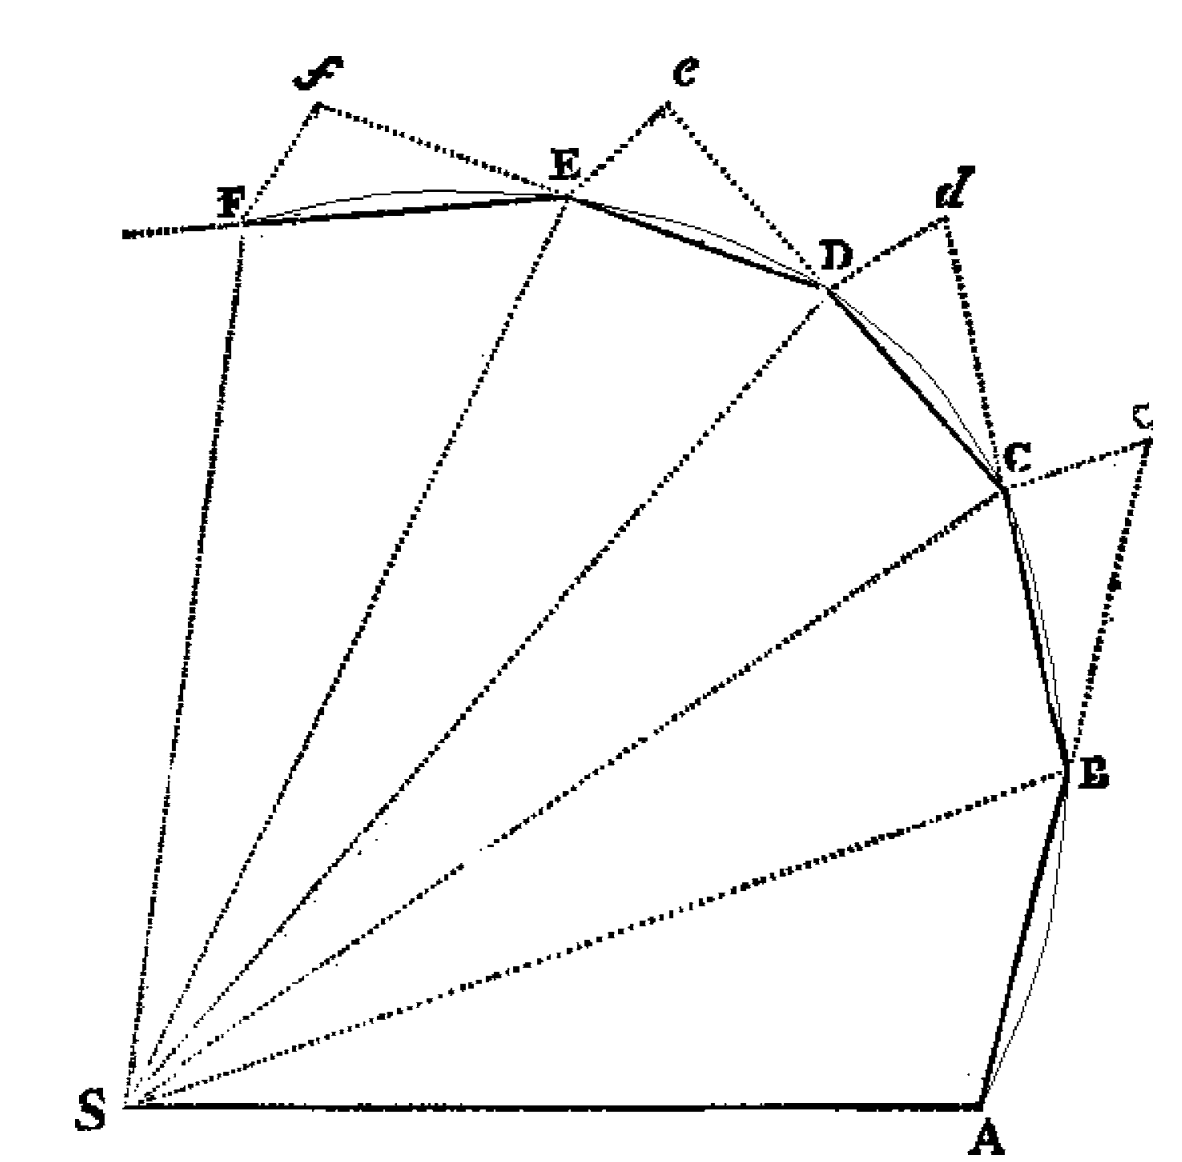
\includegraphics[width=0.5\linewidth]{newtonArea.png}
  \caption{Newton's area theorem construction, reproduced from \cite{newton1687principia}. Because it is an original 1687 diagram, it naturally looks coarse/ancient, but the geometric idea is clear.}
  \label{fig:newton-area}
\end{figure}

Approximate the orbit by a broken line $ABCDEF\cdots$ traversed in equal time steps, with instantaneous ``impulses'' at the vertices. Fix the point $S$ about which areas are swept. If there is no impulse at $B$, then after $AB$ the motion would continue straight to a point $c$ on the extension of $AB$ with $Bc=AB$. Newton's construction draws through $c$ a line parallel to $SB$ and places $C$ on this line so that $C\in SC$ (see \Cref{fig:newton-area}); this makes the successive swept triangles $\triangle SAB$ and $\triangle SBC$ have equal areas. Conversely, if equal areas are swept in equal times, then at each vertex the ``jump'' from the straight continuation (e.g., from $c$ back to $C$) must lie along $BS$ (and similarly at $C,D,\ldots$). In the smooth limit, the acceleration is therefore always directed along $AS$, i.e., the force is \emph{centripetal} with center $S$.

Thus it remains to determine the magnitude of the centripetal acceleration $a(r)$.

\section{Auxiliary circle and the affine map}

Let $\ell$ be the major axis and let $O$ be the center of the ellipse. Recall that the ellipse has semi-major axis $a$ and semi-minor axis $b$. Consider the \emph{major-axis circle} $\mathcal C$: the circle centered at $O$ with radius $a$ (so its diameter equals the major axis length $2a$). This is also the standard \emph{auxiliary circle} associated to the ellipse.

Define the affine map $\Phi$ geometrically as follows. For any point $P$ in the plane, let $P_T$ be the foot of the perpendicular from $P$ to $\ell$. On the same perpendicular line $P_TP$ choose a point $P_0$ on the same side of $\ell$ as $P$ such that
\begin{equation}
  P_TP_0=\frac{b}{a}\,P_TP.
\end{equation}
Then set $\Phi(P):=P_0$.

Equivalently, $\Phi$ fixes $\ell$ pointwise and scales all lengths perpendicular to $\ell$ by the constant factor $b/a$. This map sends lines to lines, preserves parallelism, and scales all areas by $b/a$. In the standard auxiliary circle construction, $\Phi$ maps $\mathcal C$ to the ellipse.

\paragraph{Tangents via secants (Newton's viewpoint).}
Newton often treats a tangent as the \emph{ultimate position} of a secant: if $A$ is a point on the curve and $B$ is a nearby point, then the chord line $AB$ approaches the tangent line at $A$ as $B\to A$ (in Newton's language, as one takes the ``ultimate ratio''). In our setting this provides an alternative justification for the fact that $\Phi$ carries circle tangents to ellipse tangents.

Indeed, let $A_0\in\mathcal C$ correspond to $A=\Phi(A_0)$ on the ellipse, and let $B_0\in\mathcal C$ correspond to $B=\Phi(B_0)$. Since $\Phi$ is affine, it maps the secant (chord) line $A_0B_0$ to the secant line $AB$, and it preserves incidences and parallelism. As $B_0\to A_0$, the secant line $A_0B_0$ approaches the tangent to $\mathcal C$ at $A_0$, while $AB$ approaches the tangent to the ellipse at $A$. Therefore, in the same limiting (secant-to-tangent) sense, $\Phi$ maps the circle tangent at $A_0$ to the ellipse tangent at $A$.

\begin{figure}[t]
  \centering
  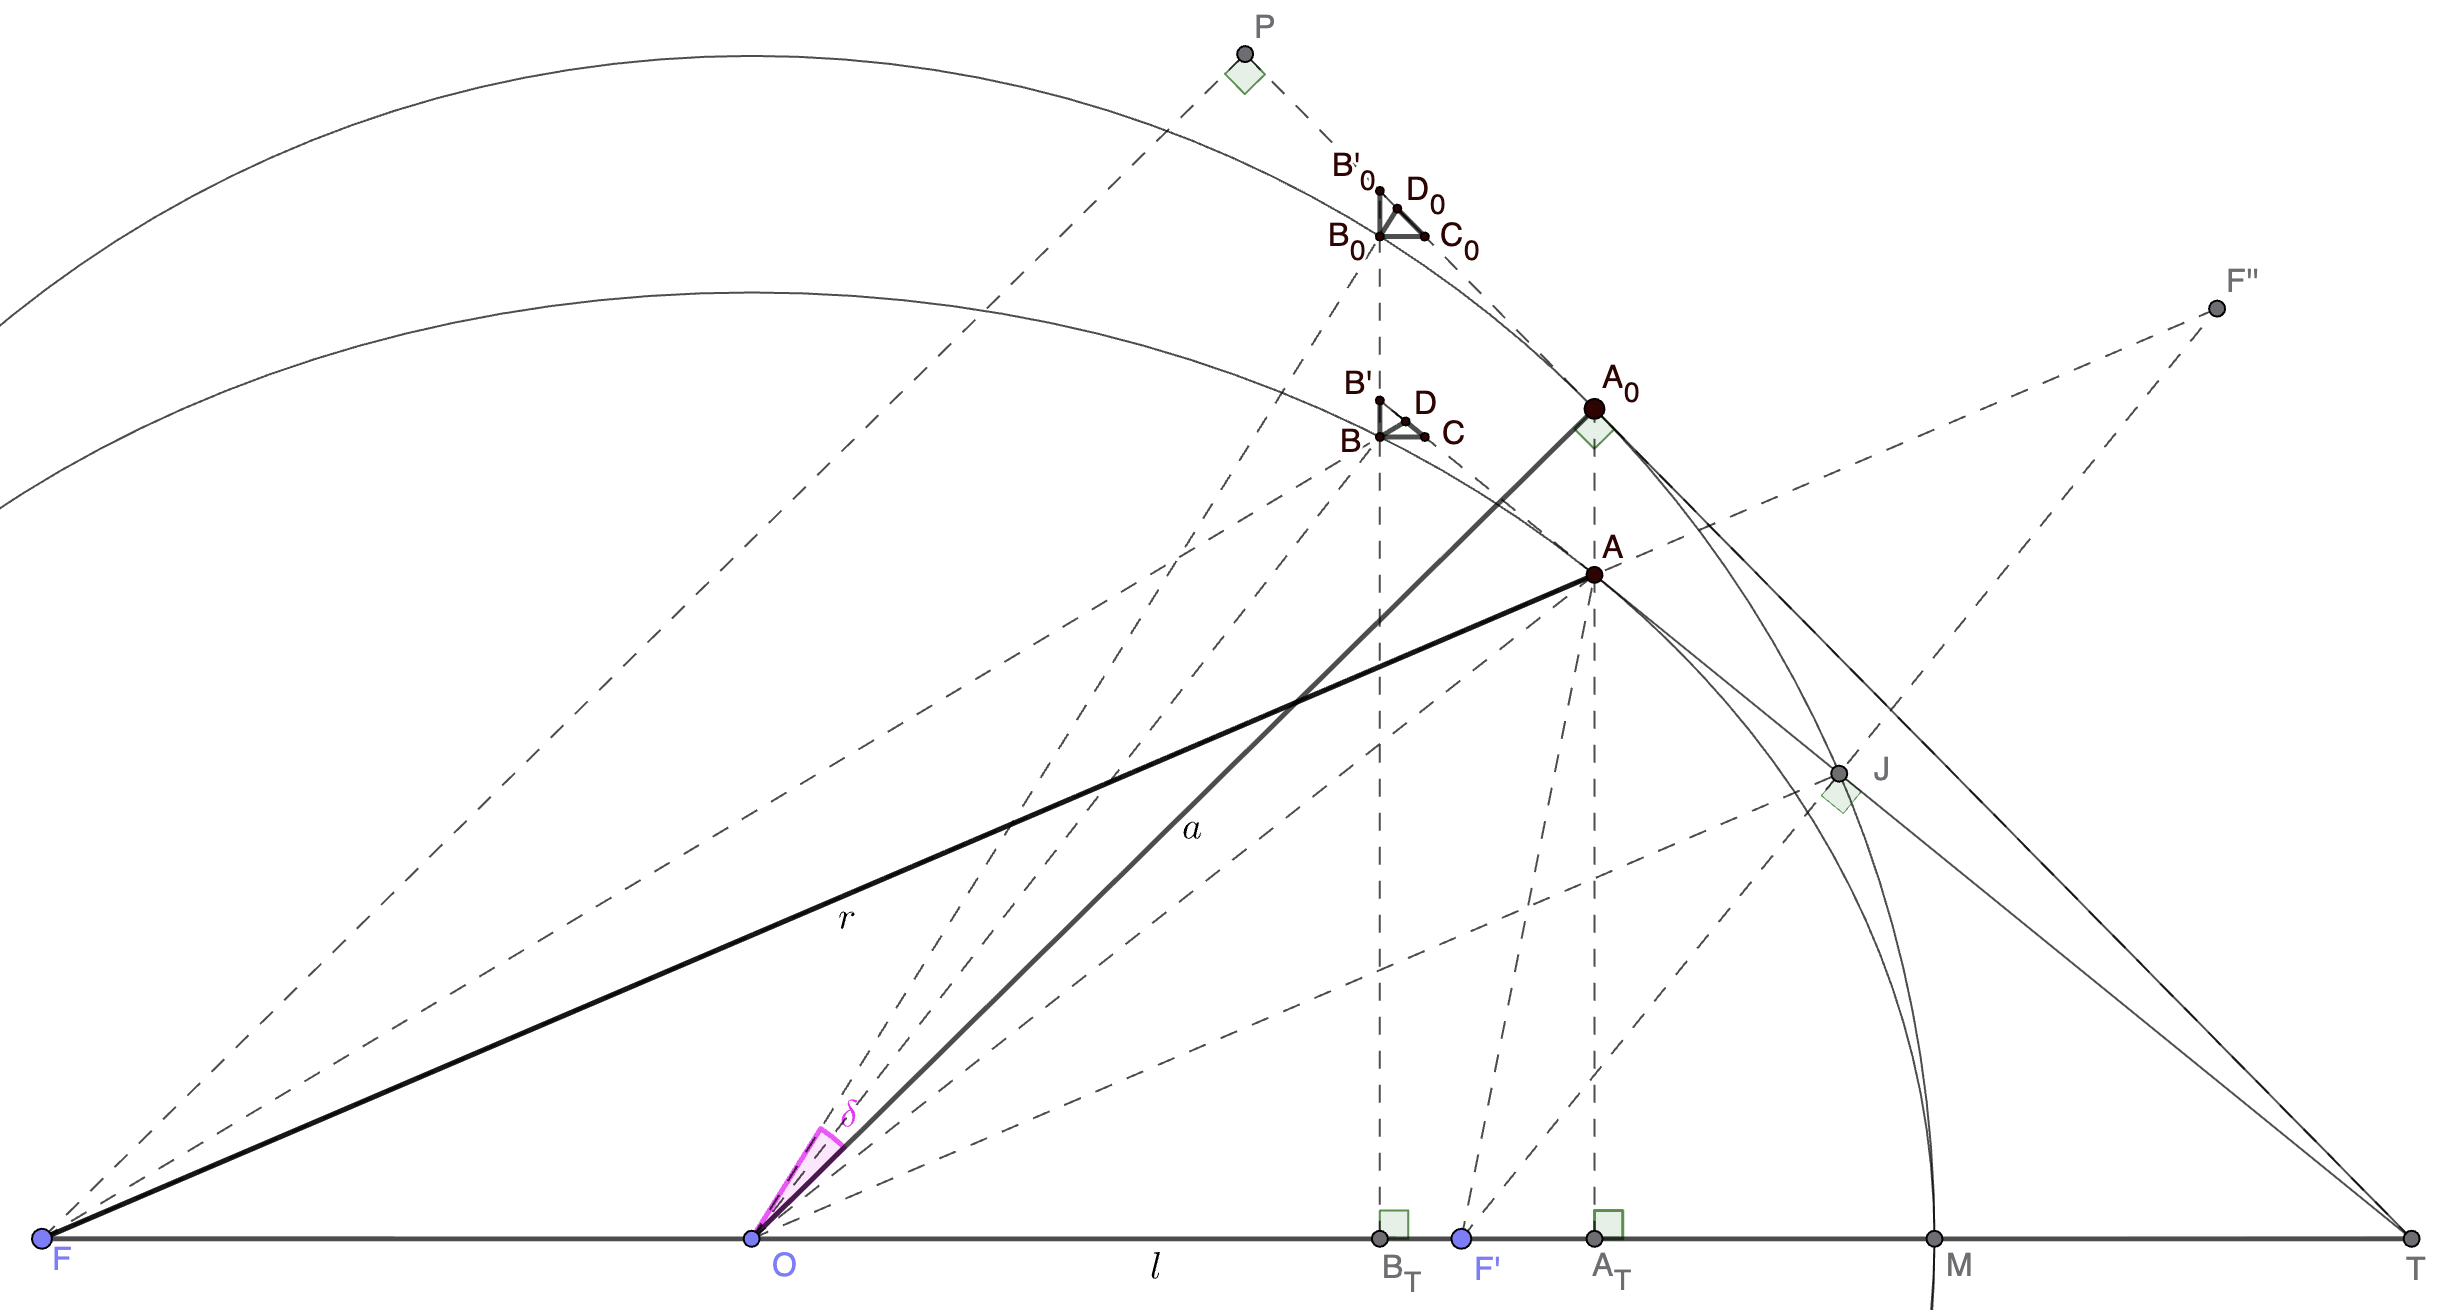
\includegraphics[width=1.1\linewidth]{MotionFigure.png}
  \caption{Affine relation of motion between the auxiliary circle and the ellipse.}
  \label{fig:affine-relation-of-motion}
\end{figure}

A few simple geometric consequences we use repeatedly:
\begin{itemize}
  \item Straight lines map to straight lines under $\Phi$.
  \item Horizontal lengths (parallel to $\ell$) are unchanged by $\Phi$.
  \item Vertical lengths (perpendicular to $\ell$) scale by $b/a$.
  \item Parallel lines stay parallel under $\Phi$, and ratios of lengths along such lines are unchanged by $\Phi$.
  \item Areas scale by $b/a$.
  \item The inverse map $\Phi^{-1}$ sends $\Phi(A)$ back to $A$ and scales vertical lengths by $a/b$.
\end{itemize}
Even though Newton did not describe affine transformations explicitly, he was well aware of these properties and applied them throughout his books. He also used clever polygonal approximations to treat areas under curves (a method far ahead of its time).
\section{Tangent transfer and matching normal drops}

We record a concrete straightedge-and-compass configuration that makes the affine ``transport'' of the short-time normal departure from the tangent completely explicit.

\subsection{Circle companions and tangent transfer}

Let $\ell$ be the major axis, then $\phi$ map a auxiliary circle $\mathcal{C}$ to the ellipse. From $A$ and $B$ drop perpendiculars to $\ell$ and extend these same vertical lines to meet the auxiliary circle $\mathcal C$ at $A_0$ and $B_0$ (choose the intersections on the same side of $\ell$ as $A$ and $B$). By construction, $\Phi(A_0)=A$ and $\Phi(B_0)=B$.
Draw the tangent to $\mathcal C$ at $A_0$ and let it meet $\ell$ at $T$.

\begin{lemma}[Tangent transfer with fixed $T$]
  \label{lem:tangent-transfer}
  Under $\Phi$, the circle tangent at $A_0$ maps to the ellipse tangent at $A$. Moreover, since $\Phi$ fixes $\ell$ pointwise, the intersection point $T\in\ell$ is the same for both tangents.
\end{lemma}
\begin{proof}
  $TA_0$ is the tangent to the circle at $A_0$. For points $B_0$ on the circle taken sufficiently near $A_0$, all such $B_0$ lie on the same side of the line $TA_0$.

  The affine bijection $\Phi$ sends lines to lines and half-planes to half-planes, so it preserves the relation ``lying on the same side of a line.'' Hence the line $\Phi(T)\Phi(A_0)$ meets the ellipse at $A=\Phi(A_0)$. Since $\Phi(T)=T$ and all nearby image points $B=\Phi(B_0)$ lie on one side of $TA$, the line $TA$ is tangent to the ellipse at $A$.

  Here we implicitly use the fact that a conic is smooth and therefore has a unique and well-defined tangent line at each point.\qedhere
\end{proof}

\subsection{The $B,C,D$ construction (ellipse and circle)}

Define $C$ as the intersection of the ellipse tangent $TA$ with the line through $B$ parallel to $\ell$, and define $D:=TA\cap FB$. Likewise, on the circle tangent $TA_0$ define $C_0$ as the intersection with the line through $B_0$ parallel to $\ell$, and define $D_0:=TA_0\cap OB_0$. By construction, $BC\parallel\ell$ and $B_0C_0\parallel\ell$.

\subsection{The point $J$ is on $\mathcal{C}$}

Extend the ray $AF$ beyond $A$ and mark a point $F''$ on this ray such that $AF''=AF'$ (so $\triangle AF'F''$ is isosceles). Let $J:=AT\cap F'F''$.

\begin{lemma}[Ellipse tangent bisects the focal angle]
  The tangent line $AT$ bisects $\angle F''AF'$.
\end{lemma}

In particular (by the isosceles geometry), $AT\perp F'F''$ and $J$ is the midpoint of $F'F''$. But we also know $O$ bisects $FF'$, so $OJ\parallel FA$ and $OJ=FF''/2=a$, which proves $J$ only to select a circle $\mathcal{C}$.

\subsection{Matching the normal drops}

The triangle similarity relations in the tangent line through $T$ give
\begin{equation}
  B_0D_0 = B_0C_0\,\frac{OD_0}{OT},
  \qquad
  BD = BC\,\frac{FD}{FT}.
\end{equation}
Dividing and using that $\Phi(B_0)=B$ and $\Phi$ maps the line through $B_0$ parallel to $\ell$ to the line through $B$ parallel to $\ell$ (since $\Phi$ fixes $\ell$ and preserves parallelism), while also mapping the tangent line $TA_0$ to $TA$, we have $\Phi(C_0)=C$. Hence the horizontal segment $B_0C_0$ is carried to $BC$, and since $\Phi$ preserves horizontal lengths, $B_0C_0=BC$.
\begin{equation}
  \frac{B_0D_0}{BD}=\frac{OD_0}{OT}\cdot\frac{FT}{FD}.
\end{equation}
Letting $B\to A$ (so $D_0\to A_0$ and $D\to A$), we obtain
\begin{equation}
  \lim_{B\to A}\frac{B_0D_0}{BD}=\frac{OA_0}{OT}\cdot\frac{FT}{FA}.
\end{equation}

\begin{proposition}[Matching drops]
  \label{prop:matching-drops}
  In the infinitesimal-step limit, the circle and ellipse normal drops from the tangent agree:
  \begin{equation}
    \boxed{\;\lim_{B\to A}\frac{B_0D_0}{BD}=1.\;}
  \end{equation}
\end{proposition}
\begin{proof}
  Now $F,O,T\in\ell$, and by construction $J\in AT$ and $OJ\parallel FA$. Hence triangles $\triangle TFA$ and $\triangle TOJ$ are similar. Therefore
  \[
    \frac{FT}{FA}=\frac{OT}{OJ}.
  \]
  Since $A_0,J\in\mathcal C$ we have $OA_0=OJ=a$, and consequently the right side of (5)
  \[
    \frac{OA_0}{OT}\cdot\frac{FT}{FA}=\frac{a}{OT}\cdot\frac{OT}{a}=1.
  \]
  which proves (6).
\end{proof}

\subsection{Transporting swept area from the ellipse to the circle}
\label{sec:transport-and-sagitta}

Let $A$ be the current point on the ellipse and $B$ the position after a small time increment $t$. Let the swept area about the focus be
\begin{equation}
  S = \operatorname{area}(\triangle F A B)=\frac{L}{2}\,t.
\end{equation}

We compare this to a corresponding small triangle on the circle. Let
\begin{equation}
  S_0 := \operatorname{area}(\triangle O A_0 B_0),
\end{equation}
two geometric scalings relate $S$ and $S_0$:
\begin{enumerate}
  \item \textbf{Height scaling from $O$ to $F$.} In the construction used in our discussion, the line through $F$ parallel to a fixed circle radius implies that the perpendicular height from $F$ to the chord $AB$ is $(r/a)$ times the perpendicular height from $O$ to the same chord direction. Hence
    \begin{equation}
      \operatorname{area}(\triangle F A B)=\frac{r}{a}\,\operatorname{area}(\triangle O A B).
    \end{equation}

  \item \textbf{Affine area scaling.} Since $\Phi$ scales area by $b/a$,
    \begin{equation}
      \operatorname{area}(\triangle O A B)=\frac{b}{a}\,\operatorname{area}(\triangle O A_0 B_0)=\frac{b}{a}\,S_0.
    \end{equation}
\end{enumerate}

Combining,
\begin{equation}
  S=\operatorname{area}(\triangle F A B)=\frac{r}{a}\cdot\frac{b}{a}\,S_0=\frac{rb}{a^2}\,S_0,
\end{equation}
so
\begin{align}
  S_0 &= \frac{a^2}{rb}\,S
  = \frac{a^2}{rb}\cdot \frac{L}{2}\,t
  = \frac{L a^2}{2 b r}\,t.
\end{align}

\subsection{Circle tangent + sagitta}
\label{subsec:sagitta}

As $B_0\to A_0$, \eqref{12} gives
\begin{equation}
  A_0D_0 = \frac{2S_0}{a}=
  \frac{2}{a}\cdot\frac{L a^2}{2 b r}\,t
  =\frac{L a}{b r}\,t.
\end{equation}

Now use elementary circle geometry relating the \emph{normal drop} from the circle to its tangent (the sagitta). For a circle of radius $a$, the perpendicular distance from the circle point reached to the tangent line satisfies (to leading order)
\begin{equation}
  B_0D_0 \approx \frac{(A_0D_0)^2}{2a}.
\end{equation}
Substituting \eqref{13} gives
\begin{equation}
  B_0D_0 \approx \frac{1}{2a}\left(\frac{L a}{b r}t\right)^2
  = \frac{L^2 a}{2 b^2 r^2}\,t^2.
\end{equation}

\subsection{From circle acceleration to ellipse acceleration}
\label{subsec:circle-to-ellipse-accel}

In the smooth limit, the \emph{normal displacement from the tangent} is precisely the drop $BD=\tfrac12 a_F\,t^2$, where $a_F$ is the magnitude of the focus-directed acceleration at $A$. Substituting the sagitta estimate (15) and equating it with $BD$ using \Cref{prop:matching-drops}, we obtain
\[
  \tfrac12 a_F\,t^2 \approx \frac{L^2 a}{2 b^2 r^2}\,t^2.
\]
Cancelling $\tfrac12 t^2$ yields
\begin{equation}
  a_F=\frac{L^2 a}{b^2}\cdot\frac{1}{r^2}.
\end{equation}

Together with Section~2 (direction toward $F$), we obtain the inverse-square central law:
\begin{equation}
  \boxed{\;\mathbf a_F(r) = -\mu\,\frac{\mathbf r}{r^3},\qquad \mu=\frac{L^2 a}{b^2}\;}
\end{equation}
where $\mathbf r$ is the position vector from $F$.

Using the ellipse identity $p=b^2/a$ (the \emph{semi-latus rectum}), this can be written in the standard Newtonian form
\begin{equation}
  \mu=\frac{L^2}{p},\qquad \mathbf a = -\frac{L^2}{p}\,\frac{\mathbf r}{r^3}.
\end{equation}
Here $\mu$ is a single positive constant, commonly called the \emph{standard gravitational parameter}; in the usual physical notation one writes $\mu=GM$ (cf. \cite{chandrasekhar1995principia,goodstein1996feynman}).

This also makes explicit how the \emph{shape} of the ellipse and the constant areal rate determine the physical parameter. Since $L=2k$ and $\mu=L^2/p$, we have
\begin{equation}
  \mu = \frac{(2k)^2}{p} = \frac{4k^2}{p}.
\end{equation}
Writing the semi-latus rectum as $p=b^2/a=a(1-e^2)$, this becomes
\begin{equation}
  \mu = \frac{L^2}{a(1-e^2)}.
\end{equation}
Equivalently, for a given inverse-square strength $\mu=GM$ and ellipse parameter $p$, the area-law constant is fixed by $k=\tfrac12\sqrt{\mu p}$ (so the orbit's geometry and the gravitating mass together determine the swept-area rate).

\section{An alternative auxiliary-circle proof (same inverse-square law)}
\label{sec:alternative-proof}

In this section we give a second derivation of the same $1/r^2$ law, still using the auxiliary circle $C$ (center $O$, radius $a$), but emphasizing a different set of local ellipse facts so that the argument has as few moving parts as possible.

\begin{figure}[t]
  \centering
  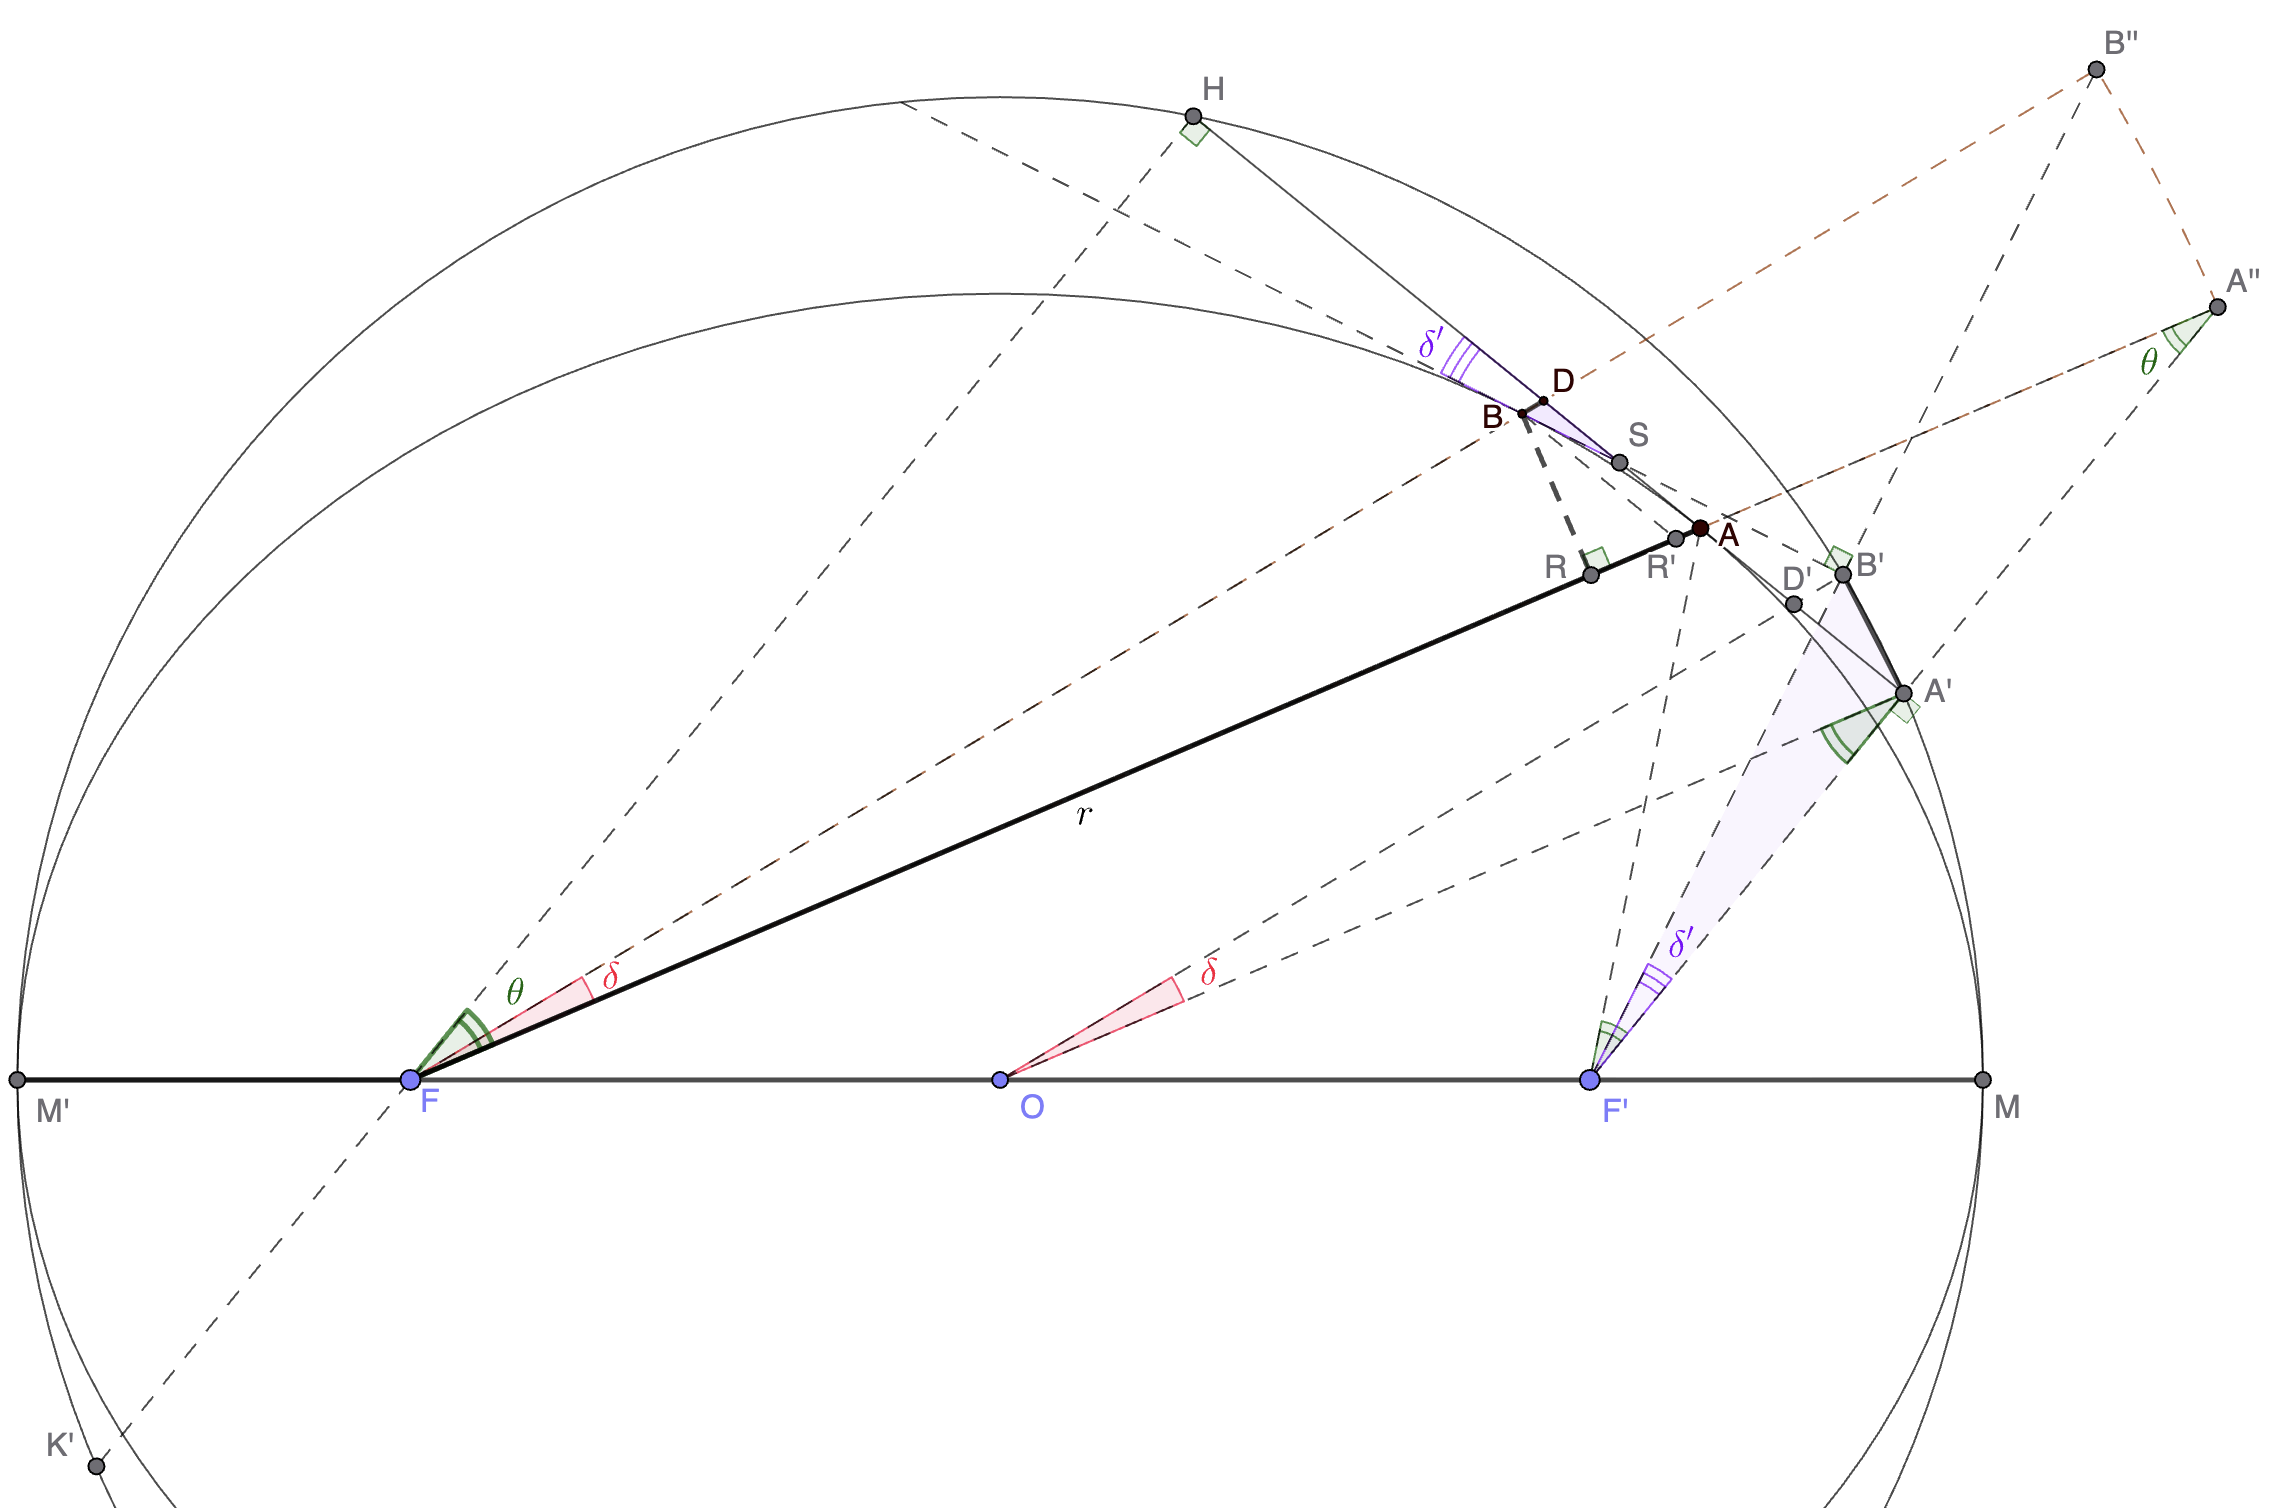
\includegraphics[width=1.1\linewidth]{proof2_1.png}
  \caption{Alternative auxiliary-circle construction used in Section~\ref{sec:alternative-proof}.}
  \label{fig:proof2-1}
\end{figure}

\subsection{Setup (only what we use)}

Let the ellipse have foci $F,F'$. Fix a point $A$ on the ellipse and write $r=FA$.
Let the tangent at $A$ meet the auxiliary circle again at $A'$. For a nearby point $B$ on the ellipse, let its tangent meet the same auxiliary circle at $B'$. We let $B\to A$.

Let $D$ be the intersection point on the tangent construction (as in \Cref{fig:proof2-1}), and let $R$ be the foot used to form the small segment $BR$ (the small transverse piece in the right triangle at $R$).

\subsection{Two standalone lemmas}

\begin{lemma}[Product identity]
  \label{lem:product-identity}
  With the notation of \Cref{fig:proof2-1},
  \begin{equation}
    FH\cdot F'\!A'=(a-c)(a+c)=b^2,
  \end{equation}
  where $c=OF$ is the focal distance (so $a^2=b^2+c^2$).
\end{lemma}

\begin{proof}
  Since $FK' \parallel F'A'$ in the construction, triangles with corresponding sides along these parallels are similar, and the segment on the parallel through $F$ has the same length as the corresponding segment on the tangent through $F'$. In particular,
  \begin{equation}
    F'\!A' = FK'.
  \end{equation}
  Therefore
  \begin{equation}
    FH\cdot F'\!A' = FH\cdot FK' = (a-c)(a+c)=a^2-c^2=b^2,
  \end{equation}
  which is the standard ellipse identity.
\end{proof}

\begin{lemma}[Newton small-distance lemma]
  \label{lem:newton-small-distance}
  As $B\to A$, the little segments cut off by nearby tangents/secants agree to first order; thus the similar-triangle relations used below are valid in the Newtonian ``ultimate ratio'' sense (any error is higher order and vanishes in the limit).
\end{lemma}

\subsection{Proof 2 (inverse-square law)}

\paragraph{Step 1: a similarity formula for $BD$.}
As $B\to A$, similarity of the indicated triangles in \Cref{fig:proof2-1} gives
\begin{equation}
  \triangle SDB \sim \triangle F'\!A'B'
  \qquad\Longrightarrow\qquad
  BD=\frac12\,AD\cdot\frac{A'B'}{A'F'}.
\end{equation}
(The factor $1/2$ is the same midpoint/evanescent factor as in the earlier Newton-style tangent-departure setup.)

In particular, this step highlights again the pair of similar triangles $\triangle F'\\!A'B'$ and $\triangle SDB$ that drives the computation.

\paragraph{Step 2: express both $AD$ and $A'B'$ in terms of $BR$.}
From the focal-geometry similarity in the figure,
\begin{equation}
  AD=\frac{AF}{FH}\,BR=\frac{r}{FH}\,BR.
\end{equation}
From the auxiliary-circle similarity (equivalently, the affine scaling ellipse $\leftrightarrow$ circle),
\begin{equation}
  A'B'=\frac{OA'}{F'\!A}\,BR=\frac{a}{r}\,BR.
\end{equation}

\paragraph{Step 3: multiply and collapse.}
Substituting the two expressions into the $BD$ formula yields
\begin{align}
  BD
  &=\frac12\left(\frac{r}{FH}BR\right)\left(\frac{a}{r}BR\right)\frac{1}{A'F'}\\
  &=\frac12\,a\,\frac{BR^2}{FH\cdot A'F'}.
\end{align}
Using \Cref{lem:product-identity} (so that $FH\cdot A'F'=b^2$) we obtain
\begin{equation}
  BD=\frac12\,a\,\frac{BR^2}{b^2}.
\end{equation}

Finally, using the standard ellipse identity $p=b^2/a$ (the semi-latus rectum), one may rewrite the above in the equivalent form
\begin{equation}
  BD=\frac{1}{2p}\,BR^2,
\end{equation}
which is the same local ``departure from the tangent'' scaling used earlier, hence leads again (via the same $BD=\tfrac12 a_F (\Delta t)^2$ identification and $BR\cdot r = L\,\Delta t$) to the inverse-square law.
\hfill$\square$

\subsection{Proof 3 (hodograph-style computation)}
\label{subsec:proof3-hodograph}

From \Cref{lem:product-identity},
\begin{equation}
  F'\!A'=\frac{b^2}{FH}.
\end{equation}
Let $v=\lvert \mathbf v\rvert$ be the speed at $A$. Since the velocity direction is tangent to the orbit and $FH$ is perpendicular to that tangent (as in the construction), the areal-rate constant gives
\begin{equation}
  FH\cdot v = L.
\end{equation}
Combining,
\begin{equation}
  F'\!A'=\frac{b^2}{FH}=\frac{v\,b^2}{L}.
\end{equation}
For two nearby points $A,B$ we therefore have, in the Newtonian small-step sense,
\begin{equation}
  A'B'=\Delta(F'\!A')=\frac{b^2}{L}\,\Delta v
  =\frac{b^2}{L}\,a_F\,\Delta t,
\end{equation}
where $a_F$ is the magnitude of the (focus-directed) acceleration and $\Delta v\approx a_F\Delta t$.
On the other hand, from the auxiliary-circle similarity used above,
\begin{equation}
  A'B'=\frac{OA'}{F'\!A}\,BR=\frac{a}{r}\,BR.
\end{equation}
Eliminating $A'B'$ gives
\begin{equation}
  a_F=\frac{L}{b^2}\,\frac{A'B'}{\Delta t}.
\end{equation}
Next, using again the auxiliary-circle similarity $A'B'=\frac{a}{r}BR$ and the areal law $BR=L\,\Delta t/r$ (as in Section~5), we have
\begin{equation}
  A'B'=\frac{a}{r}\,\frac{L\,\Delta t}{r}
  =\frac{a}{r^2}\,L\,\Delta t.
\end{equation}
Combining equations~(6.18)--(6.19) yields
\begin{equation}
  a_F=\frac{L^2}{p}\,\frac{1}{r^2}.
\end{equation}
exactly the same inverse-square formula as in equations~(5.14)--(5.15).
\hfill$\square$

\subsection{Discussion: directrix circle and a hodograph viewpoint}
\label{subsec:sec6-discussion}

\paragraph{Directrix circle variant.}
One can re-run essentially the same similarity argument by replacing the auxiliary circle $\mathcal C$ (center $O$, radius $a$) with the \emph{directrix circle} centered at $F$ of radius $2a$ (cf.\ the construction used in Section~5).
Extending $FA$ to meet this directrix circle at $A''$, one has $A''A'F'$ colinear; similarly, extending $FB$ meets the directrix circle at $B''$ with $B''B'F'$ colinear.
Moreover, $A'$ and $B'$ are midpoints of the segments $A''F'$ and $B''F'$, respectively, so
\begin{equation}
  A''B'' = 2\,A'B'.
\end{equation}
Consequently,
\begin{equation}
  \triangle A'B'F' \sim \triangle A''B''F',
\end{equation}
and the same chain of similar-triangle identities yields the same ultimate-ratio estimate for the normal drop $BD$, hence the same inverse-square dependence.

\paragraph{Connection to Maxwell's hodograph.}
The product identity in \Cref{lem:product-identity} (already implicit in classical ellipse geometry) also appears in Maxwell's discussion of the \emph{hodograph} of planetary motion: for an inverse-square central force the velocity vector $\mathbf v(t)$ traces a circle in velocity space (Hamilton's hodograph), and Maxwell notes that this hodograph circle is similar to the directrix circle, with its ``speed origin'' at $F'$, but rotated by $90^\circ$ counterclockwise \cite{maxwell1877mattermotion}.

From this point of view, our construction may be read as relating the geometric drop $BD$ directly to a rotated hodograph circle $C$.
This suggests a third, very short proof that reproduces the same acceleration formula.

\section{Other conic sections}
\label{sec:other-conics}

Although we have focused on the elliptic (bound) case, the same inverse-square central-force setting also admits other conic-section trajectories.
Besides ellipses, the remaining possibilities are the parabola (the threshold case) and the hyperbola (the unbound case), together with a degenerate limiting case discussed next.

\subsection{A ``strange line'' (degenerate ellipse / degenerate hyperbola)}
\label{subsec:strange-line}

In the limit where a conic section ``just touches'' the cutting plane, one obtains a degenerate conic: a single line (counted with multiplicity in the projective viewpoint).
In our geometric setting it is convenient to regard this as a limiting case of the family of ellipses, but it can also be viewed as a limiting (degenerate) hyperbola.

\subsection{Hyperbola}
\label{subsec:hyperbola}

For an inverse-square central force, hyperbolic trajectories correspond to unbound motion: the point mass comes in from infinity and escapes back to infinity, with the force center located at a focus of the hyperbola.

See Figure~4 for the auxiliary-circle construction used to carry out the same inverse-square argument in the hyperbola case.
\begin{figure}[htbp]
  \centering
  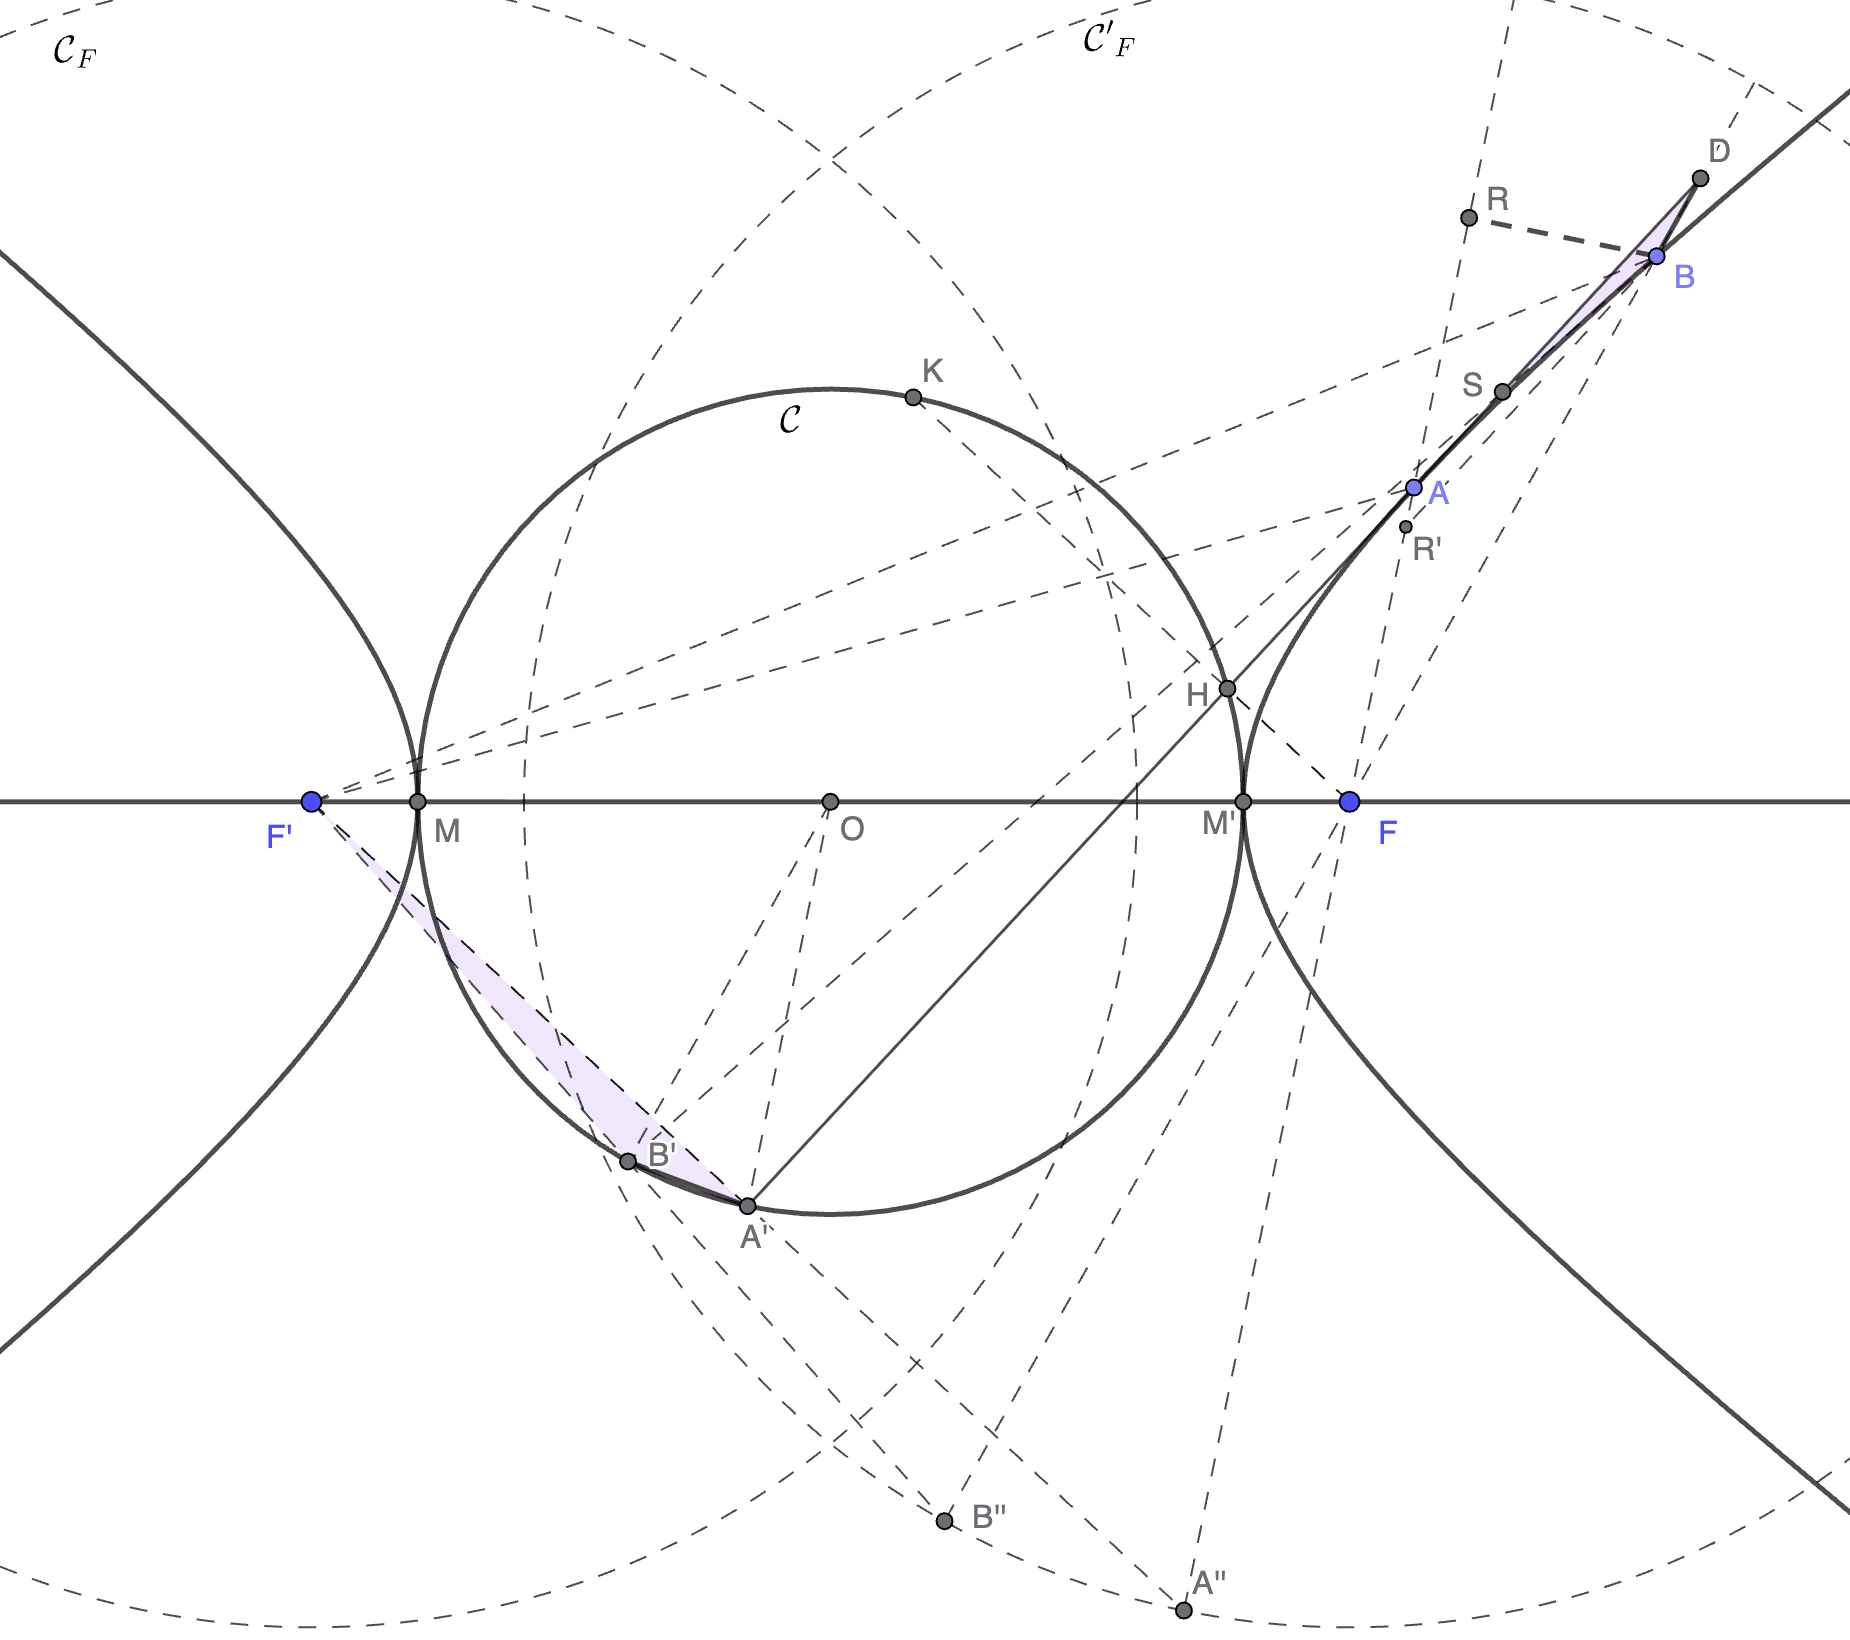
\includegraphics[width=1.1\linewidth]{hyperbola.png}
  \caption{Auxiliary-circle construction for the hyperbola case.}
  \label{fig:hyperbola}
\end{figure}
In this hyperbola setup, one may again view the auxiliary circle $\mathcal C$ as providing a convenient geometric proxy for the (circular) hodograph, with $F'$ taken as the velocity origin.
As in the elliptic case, this proxy picture must be rotated by $90^\circ$ to match the correct direction of the velocity vector in the hodograph construction.

Likewise, the directrix circle $\mathcal{C'}_{F}$ may be regarded as a $2\times$ scaling of the auxiliary circle $\mathcal C$ with scaling center $F'$; consequently it can also be interpreted as a scaled version of the hodograph, again up to the same $90^\circ$ rotation.

The same key product identity Lemma 6.1 also holds in this hyperbola setting, though processed differently
\begin{equation}
  F'\!A'\cdot FH = FH\cdot FK = F\!M'\cdot FM = (c-a)(c+a)=c^2-a^2=b^2,
\end{equation}
using the same tangent/intercept relations (here $c=OF$ and $a^2=b^2+c^2$).

Similarly, in the analogue of Proof~2 the computation is again driven by the same pair of similar triangles $\triangle F'\!A'B'$ and $\triangle SDB$.

There is also a ``swapped-focus'' situation leading to the same right-branch hyperbola: instead of an attractive (centripetal) force toward $F$, one may consider a centrifugal force directed away from $F'$ acting on the particle as it moves from $A$ to $B$.
In that case to carry out the proof, the roles of $F$ and $F'$ are interchanged, and the point $R$ is dropped onto the extension of the new line $FA$.
The points $H$ and $A'$ also exchange roles, $B'$ moves to the opposite side of the auxiliary circle $\mathcal C$, and $D$ becomes the intersection of the tangent line at $A$ with the new line $FB$ (that's $F'B$ as in Figure~4). Readers should be able to construct the modified plot accordingly without difficulty and the proof follows exactly the same.

So once Figure 4 is in place, the remaining steps corresponding to our Proofs~2 and~3 for hyperbola follow with only minor, mostly notational, changes.

\subsection{Parabola}
\label{subsec:parabola}

The parabolic trajectory is the boundary between bound (elliptic) and unbound (hyperbolic) motion.
It is also distinguished geometrically as the conic section obtained when the cutting plane is parallel to a generating edge of the cone.

One can also view a parabola as a limiting ellipse in which $a,c\to\infty$ while $(a\!-\!c)$ stays finite.
Indeed, since $p=b^2/a=(a+c)(a-c)/a$, in this limit one has $p\to 2(a-c)$.
It is therefore natural to parametrize the parabola by setting $a-c$ as a single parameter $a$, so that $p=2a$. From this perspective, the auxiliary circle degenerates to the tangent line at the vertex of the parabola, perpendicular to the symmetry axis $AF$ (with $F$ the remaining focus).

Of course, this is consistent with the polar form: the eccentricity satisfies $e=c/a=1$ for a parabola. One can similarly think of the parabola as an approximation/limit of hyperbolas as $a,c\to \infty$ while keeping $(c\!-a)$ constant.

As the eccentricity of an ellipse tends to 1, the second focus recedes to $\infty$ along the axis; in the limit it becomes a remote focus. Hence the “directrix circle” construction from the ellipse case no longer survives as a literal circle centered at the observed focus.
Yet the effect of that construction does survive: a circle of infinite radius, centered at the remote focus, degenerates into a straight line perpendicular to the axis—namely the parabola’s directrix. In this limiting viewpoint the directrix may be regarded as the remnant of the former directrix circle, positioned so that it meets the axis
$AF$ at a point symmetrically placed with respect to the vertex
$A$ (in the same sense as in the elliptical construction). So while ellipse and hyperbola each has two directrix circles and two directrix lines, parabola have only one observable directrix "circle" and and one directrix line, furthermore this circle degenerates to the same line.

However, we will also show that a parabola still admits several natural associated circles that encode useful geometry. In particular, although the earlier auxiliary circle and dirextrix circle all have degenerated into a line, one may still construct a hodograph circle of various scaling similar to what we have done in ellipse and hyperbolar, which remains genuinely circular and retains the kinematic/geometric information needed for the argument.

In this section we show that the analogues of Proofs~2 and~3 from the ellipse case also hold for the parabola, with some special care.
We recommend a read of Newton's style of argument, such as the historical collection of various properties of the parabola in \href{https://doi.org/10.5539/apr.v11n2p30}{\cite{stavek2019newtonsparabola}}.
However, a much clearer explanation of the hodograph for the parabolic case is given by \cite{derbes2001reinventing}, which uses the circle centered at the focus $F$ with radius $2a$.
With this circle, Maxwell/Hamilton's hodograph proof for the direct problem extends naturally to the parabola.

\begin{figure}[t]
  \centering
  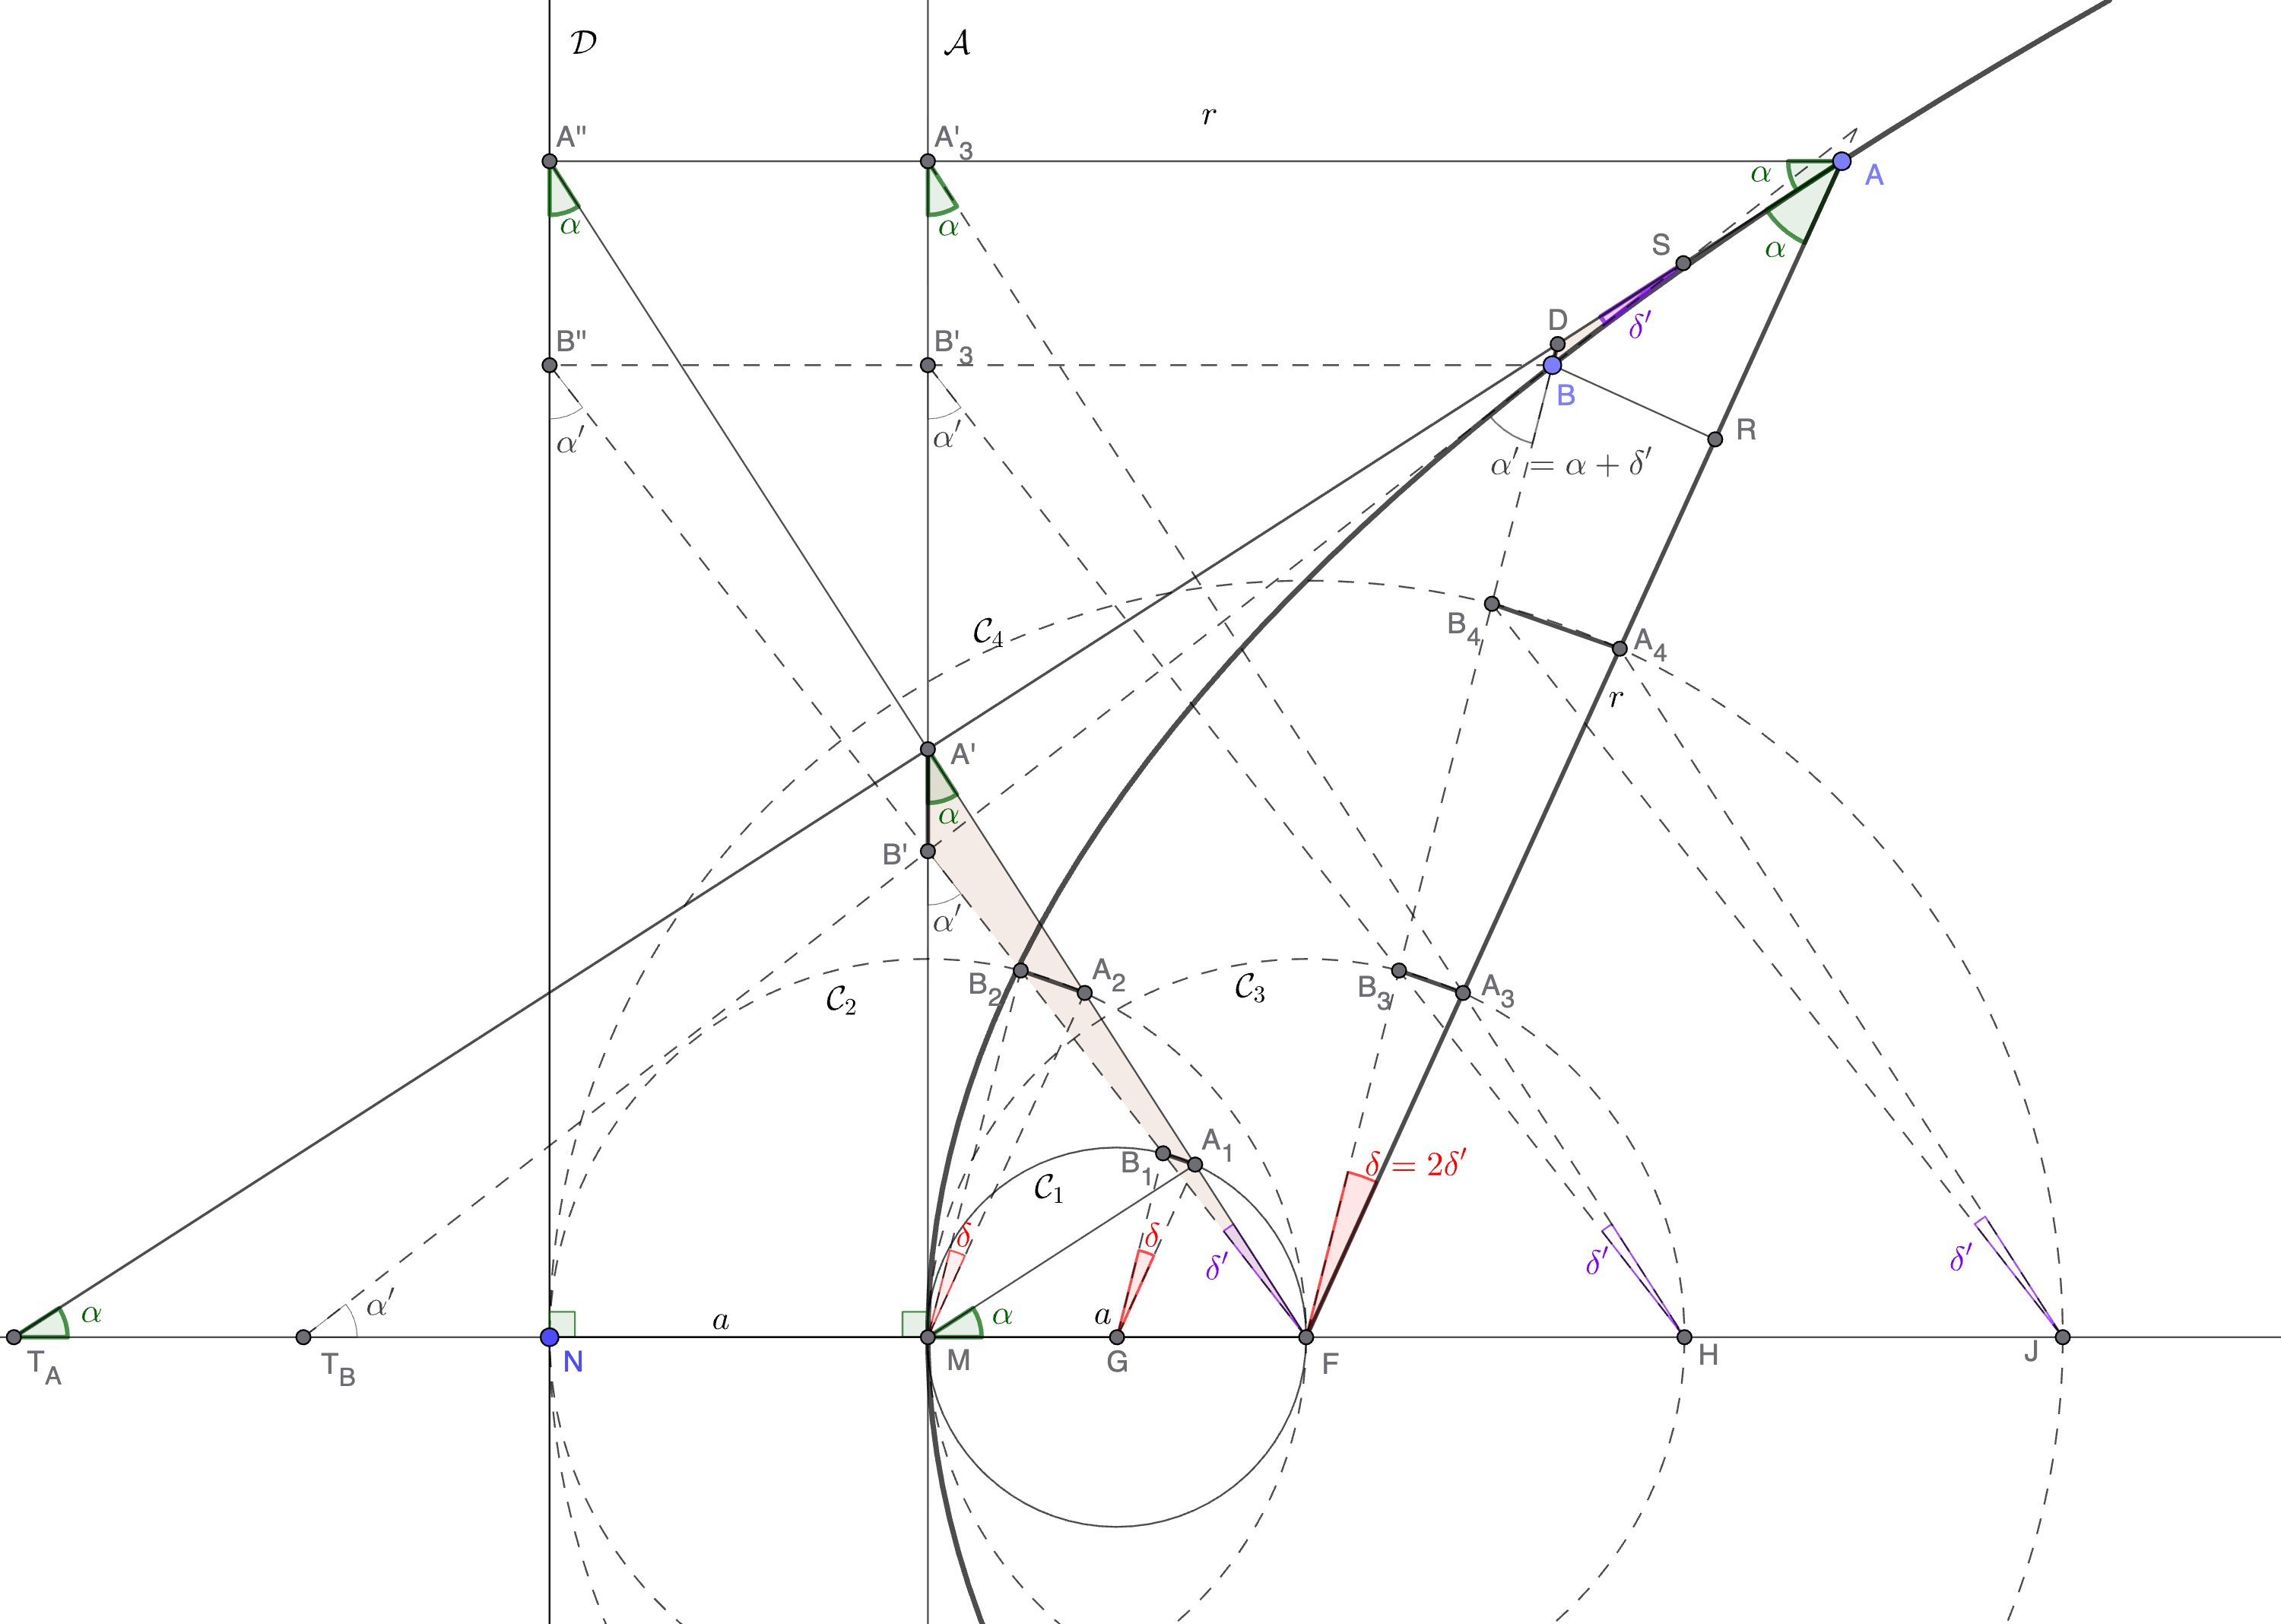
\includegraphics[width=1.1\linewidth]{parabola_2.png}
  \caption{Parabola construction used in Section~\ref{subsec:parabola} (parabola analogue of Proof~2).}
  \label{fig:parabola-proof2}
\end{figure}

\subsubsection{Parabola variant of Proof 2: a constant $BR^2/BD$}
\label{subsubsec:parabola-proof2}

We sketch a parabola analogue of Proof~2 that is closest in spirit to the auxiliary-circle computation.
Using the same Newtonian small-step interpretation as before, it is enough to show that the ratio $BR^2/BD$ tends to a \emph{constant} as $B\\to A$; this yields the same local ``departure from the tangent'' law and hence the same inverse-square conclusion.

More precisely, in the parabolic construction (with notation matching the ellipse case: $A$ current point, $B$ a nearby point, $BD$ the normal drop to the tangent at $A$, and $BR$ the short transverse segment used in the area-law step), one proves that
\begin{equation}
  \boxed{\\;\\lim_{B\\to A}\\frac{BR^2}{BD}=4a,\\;}
\end{equation}
where $a$ is the parabola parameter defined above (so that the semi-latus rectum is $p=2a$).

We now briefly indicate a geometric proof of this claim. As $B\\to A$ (so the small angles $\\delta,\\delta'\\to 0$), the similar triangles in the figure give
\begin{equation}
  \\frac{A'B'}{BD}=\\frac{B'F}{DS}\\sim \\frac{2\\,B'F}{DA}.
  \\tag{1}
\end{equation}
Resolve the last ratio using the common angle $\\alpha$:
\begin{equation}
  \\frac{B'F}{DA}
  =
  \\frac{B'F\\sin\\alpha}{DA\\sin\\alpha}
  \\sim \\frac{a}{BR}.
  \\tag{2}
\end{equation}
Here $DA\\sin\\alpha$ is the small transverse ``width'' represented by the chord $BR$, while $B'F\\sin\\alpha$ is the fixed transverse scale of the parabola, equal to $a$.
Putting (2) into (1) yields
\begin{equation}
  \\frac{A'B'}{BD}\\sim \\frac{2a}{BR},
  \\qquad\\text{so}\\qquad
  BD\\sim \\frac{A'B'\\,BR}{2a}.
  \\tag{3}
\end{equation}
But the chord $A'B'$ subtends the small angle $\\delta'$ at $F$, hence $A'B'\\sim r\\delta'$. Since in the construction one has $BR=2r\\delta'$, it follows that $A'B'\\sim \\tfrac12 BR$.
Substituting this into (3) gives
\begin{equation}
  BD\\sim \\frac{(\\tfrac12 BR)\\,BR}{2a}=\\frac{BR^2}{4a},
  \\qquad\\text{hence}\\qquad
  \\frac{BR^2}{BD}\\to 4a.
\\end{equation}

We now briefly indicate a geometric proof of this claim. As $B\\to A$ (so the small angles $\\delta,\\delta'\\to 0$), the similar triangles in the figure give
\begin{equation}
  \\frac{A'B'}{BD}=\\frac{B'F}{DS}\\sim \\frac{2\\,B'F}{DA}.
  \\tag{1}
\end{equation}
Resolve the last ratio using the common angle $\\alpha$:
\begin{equation}
  \\frac{B'F}{DA}
  =
  \\frac{B'F\\sin\\alpha}{DA\\sin\\alpha}
  \\sim \\frac{a}{BR}.
  \\tag{2}
\end{equation}
Here $DA\\sin\\alpha$ is the small transverse ``width'' represented by the chord $BR$, while $B'F\\sin\\alpha$ is the fixed transverse scale of the parabola, equal to $a$.
Putting (2) into (1) yields
\begin{equation}
  \\frac{A'B'}{BD}\\sim \\frac{2a}{BR},
  \\qquad\\text{so}\\qquad
  BD\\sim \\frac{A'B'\\,BR}{2a}.
  \\tag{3}
\end{equation}
But the chord $A'B'$ subtends the small angle $\\delta'$ at $F$, hence $A'B'\\sim r\\delta'$. Since in the construction one has $BR=2r\\delta'$, it follows that $A'B'\\sim \\tfrac12 BR$.
Substituting this into (3) gives
\begin{equation}
  BD\\sim \\frac{(\\tfrac12 BR)\\,BR}{2a}=\\frac{BR^2}{4a},
  \\qquad\\text{hence}\\qquad
  \\frac{BR^2}{BD}\\to 4a.
\\end{equation}

This is the direct parabolic counterpart of equation~(6.10) in the elliptic setting: once the constant ratio $BR^2/BD$ is established, the remainder of the argument (identifying $BD\\approx \\tfrac12 a_F(\\Delta t)^2$ and using the area-law relation $BR\\cdot r=L\\,\\Delta t$) proceeds exactly as before, and therefore again yields $a_F\\propto 1/r^2$.

\section{Summary}
We hope this alternative proof of the inverse-square law is accessible to young readers and highlights a guiding theme of the \emph{Principia}: one can reach deep dynamical conclusions from elementary geometry.

As Feynman put it, ``It is not easy to use the geometrical method to discover things. It is very difficult, but the elegance of the demonstrations after the discoveries are made is really very great. The power of the analytic method is that it is much easier to discover things than to prove things. But not in any degree of elegance. It's a lot cancellations and so on.''

\bibliographystyle{alphaurl}
\bibliography{references}

\end{document}
